 \documentclass[12pt,a4paper]{article}

\usepackage{graphicx}% Include figure files
\usepackage{dcolumn}% Align table columns on decimal point
\usepackage{bm}% bold math
%\usepackage{hyperref}% add hypertext capabilities
%\usepackage[mathlines]{lineno}% Enable numbering of text and display math
%\linenumbers\relax % Commence numbering lines

%\usepackage[showframe,%Uncomment any one of the following lines to test 
%%scale=0.7, marginratio={1:1, 2:3}, ignoreall,% default settings
%%text={7in,10in},centering,
%%margin=1.5in,
%%total={6.5in,8.75in}, top=1.2in, left=0.9in, includefoot,
%%height=10in,a5paper,hmargin={3cm,0.8in},
%]{geometry}

\usepackage{multicol}%Para hacer varias columnas
\usepackage{multicol,caption}
\usepackage{multirow}
\usepackage{cancel}
\usepackage{hyperref}
\hypersetup{
    colorlinks=true,
    linkcolor=blue,
    filecolor=magenta,      
    urlcolor=cyan,
}

\setlength{\topmargin}{-1.0in}
\setlength{\oddsidemargin}{-0.3pc}
\setlength{\evensidemargin}{-0.3pc}
\setlength{\textwidth}{6.75in}
\setlength{\textheight}{9.5in}
\setlength{\parskip}{0.5pc}

\usepackage[utf8]{inputenc}
\usepackage{expl3,xparse,xcoffins,titling,kantlipsum}
\usepackage{graphicx}
\usepackage{xcolor} 
\usepackage{siunitx}
\usepackage{nopageno}
\usepackage{lettrine}
\usepackage{caption}
\renewcommand{\figurename}{Figura}
\usepackage{float}
\renewcommand\refname{Bibliograf\'ia}
\usepackage{amssymb}
\usepackage{amsmath}
\usepackage[rightcaption]{sidecap}
\usepackage[spanish]{babel}

\providecommand{\abs}[1]{\lvert#1\rvert}
\providecommand{\norm}[1]{\lVert#1\rVert}
\newcommand{\dbar}{\mathchar'26\mkern-12mu d}

\usepackage{mathtools}
\DeclarePairedDelimiter\bra{\langle}{\rvert}
\DeclarePairedDelimiter\ket{\lvert}{\rangle}
\DeclarePairedDelimiterX\braket[2]{\langle}{\rangle}{#1 \delimsize\vert #2}

% CABECERA Y PIE DE PÁGINA %%%%%
\usepackage{fancyhdr}
\pagestyle{fancy}
\fancyhf{}

\begin{document}

Macías Márquez Misael Iván

\begin{enumerate}



%%%1%%%



\item Comprobar el principio de superposición, solo para R6

El principio de superposición establece que el efecto que dos o más fuentes tienen sobre una impedancia es igual a la suma de cada uno de los efectos de cada fuente tomados por separado, sustituyendo todas las fuentes de tensión restantes por un corto circuito, y todas las fuentes de corriente restantes por un circuito abierto\footnote{https://es.wikipedia.org/wiki/Teorema\_de\_superposici\%C3\%B3n}.

Empecemos por medir el voltaje en R6 dejando abiertas las terminales de la fuente de corriente:

\begin{figure}[h!]
    \centering
    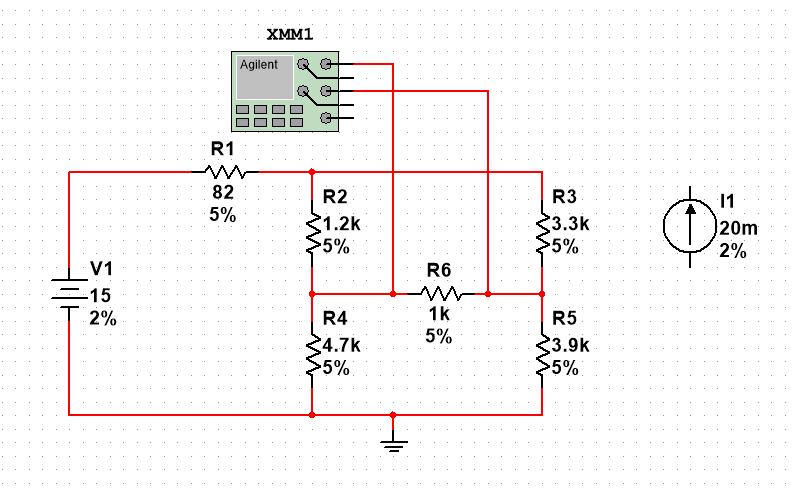
\includegraphics[scale=0.4]{1,a.PNG}

    \label{fig:my_label}
\end{figure}

\begin{figure}[h!]
    \centering
    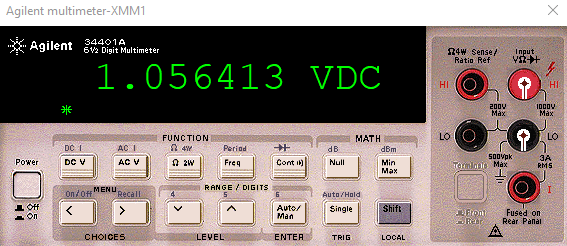
\includegraphics[scale=0.5]{1.a.multi.PNG}

    \label{fig:my_label}
\end{figure}

$\delta V_1 =(1.056413 \cdot 0.0035 + 10 \cdot 0.0005) = 0.008697 V $

y ahora sustituyendo la fuente de voltaje por un corto circuito y midiendo de nuevo el voltaje en R6:
\newpage

\begin{figure}[h!]
    \centering
    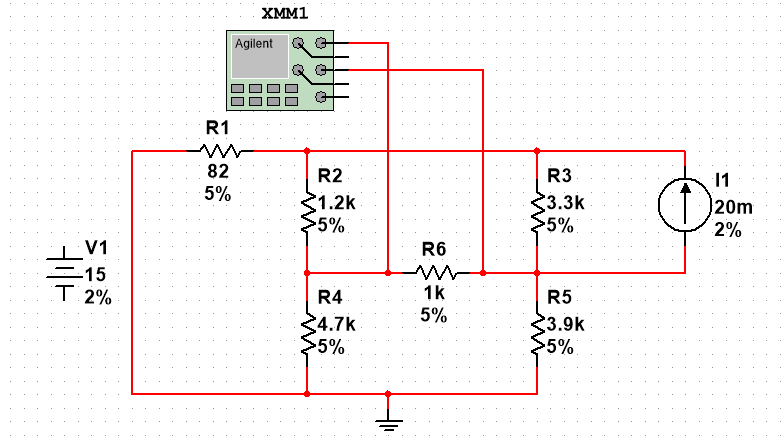
\includegraphics[scale=0.4]{1.b.PNG}

    \label{fig:my_label}
\end{figure}

\begin{figure}[h!]
    \centering
    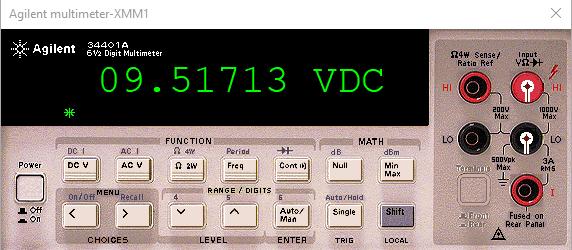
\includegraphics[scale=0.5]{1.b.multi.PNG}

    \label{fig:my_label}
\end{figure}

$\delta V_2 =(9.51713 \cdot 0.0035 + 10 \cdot 0.0005) = 0.03830 V $

Sumando los 2 voltajes obtenidos obtenemos tenemos que\footnote{Las incertidumbre reportadas son las descritas en el manual del multímetro "chrome-extension://efaidnbmnnnibpcajpcglclefindmkaj/viewer.html?pdfurl=https\%3A\%2F\%2Fwww.tme.eu\%2FDocument\%2Fadbea8905c9292cf883d5784d5c80a80\%2F34401-90420.pdf" }:

\begin{equation*}
    V_1 + V_2 = (1.0564 \pm 0.008697) V + (9.5171 \pm 0.03830) V = (10.5735 \pm 0.0470) V
\end{equation*}

El voltaje del circuito completo para la resistencia R6 es:



\begin{figure}[h!]
    \centering
    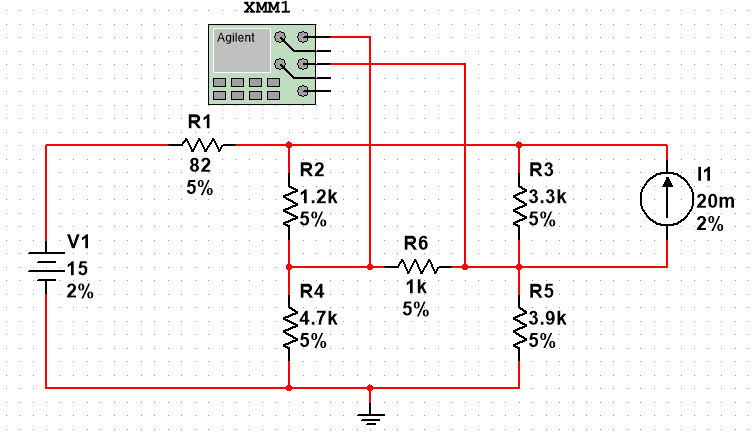
\includegraphics[scale=0.4]{1.completo.PNG}

    \label{fig:my_label}
\end{figure}

\begin{figure}[h!]
    \centering
    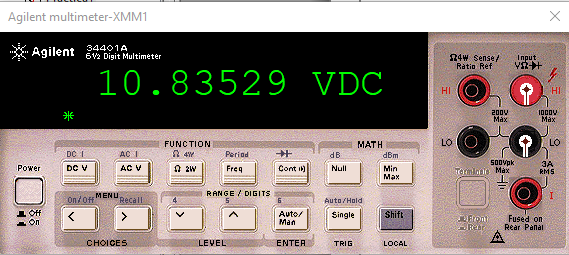
\includegraphics[scale=0.5]{1.completo.multi.PNG}

    \label{fig:my_label}
\end{figure}

lo que nos da un error relativo de $2.5\%$ y lamentablemente el error es 30 veces la incertidumbre absoluta dada por el principio de superposición por lo que se podría considerar no satisfactoria. 



\newpage
%%%2%%%



\item Medir todos los voltajes V's

Colocando un multímetro en cada componente de circuito en paralelo:

\begin{figure}[h!]
    \centering
    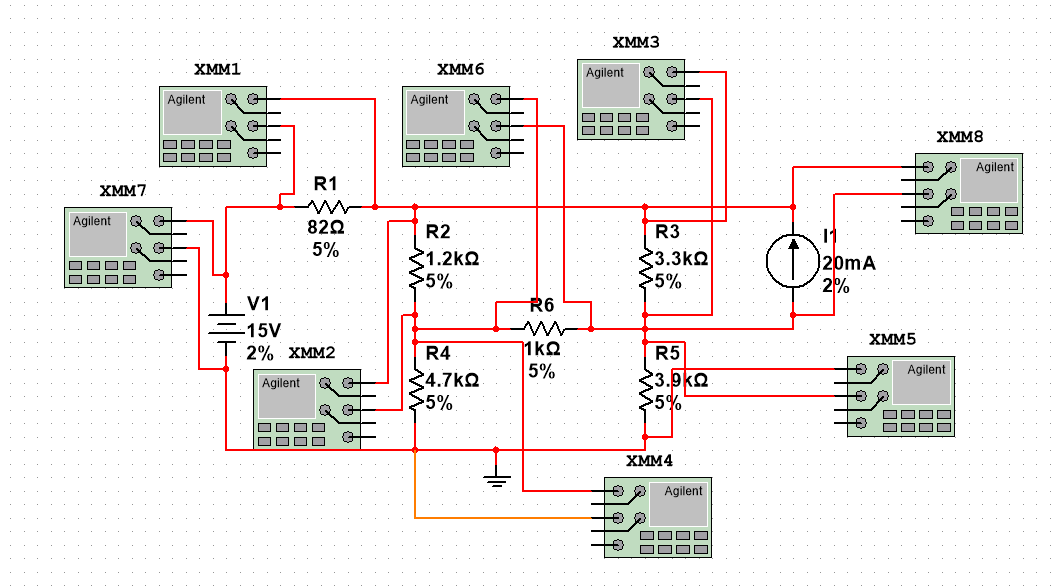
\includegraphics[scale=0.4]{circuito voltajes.PNG}
    \label{fig:my_label}
\end{figure}

nos dan los siguientes voltajes:


\begin{figure}[h!]
    \centering
    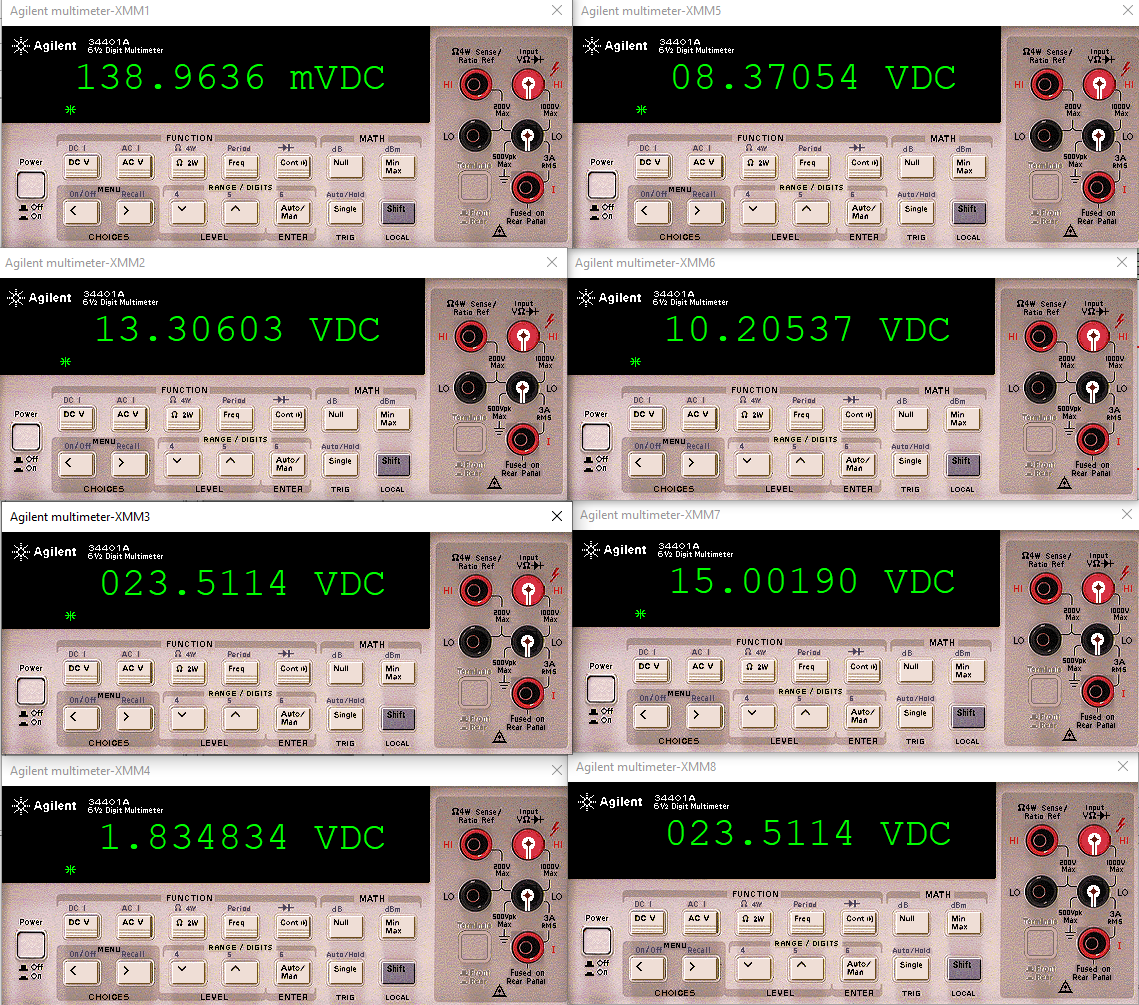
\includegraphics[scale=0.4]{voltajes medidos.PNG}
    \label{fig:my_label}
\end{figure}



\newpage
%%%3%%%



\item Medir todas las corrientes I's

En este caso se deben colocar los multímetros en serie.

\begin{figure}[h!]
    \centering
    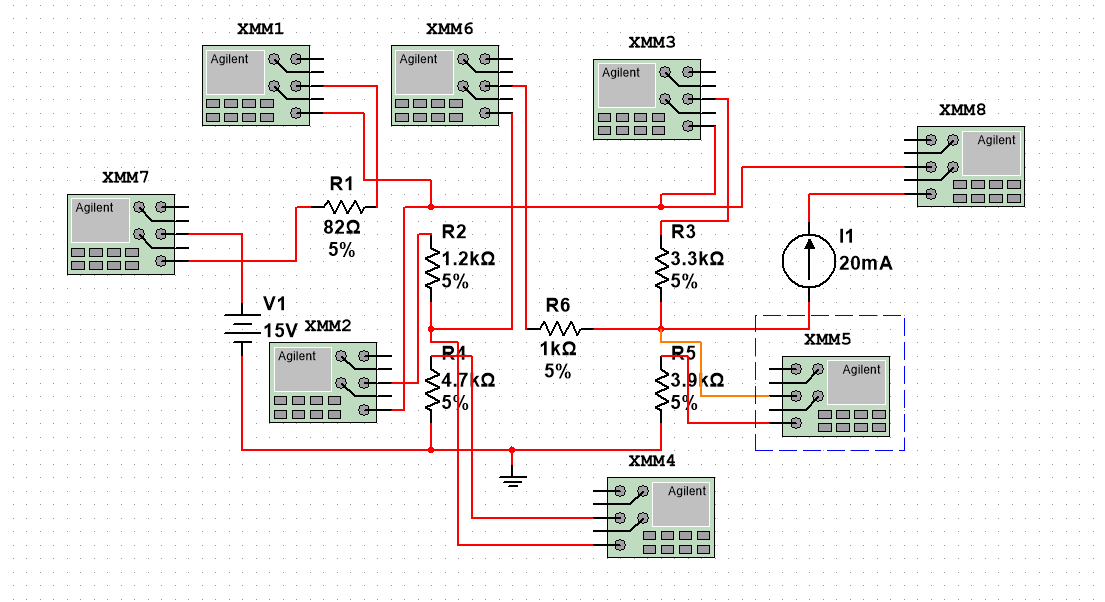
\includegraphics[scale=0.4]{circuito corrientes.PNG}
    \label{fig:my_label}
\end{figure}

\begin{figure}[h!]
    \centering
    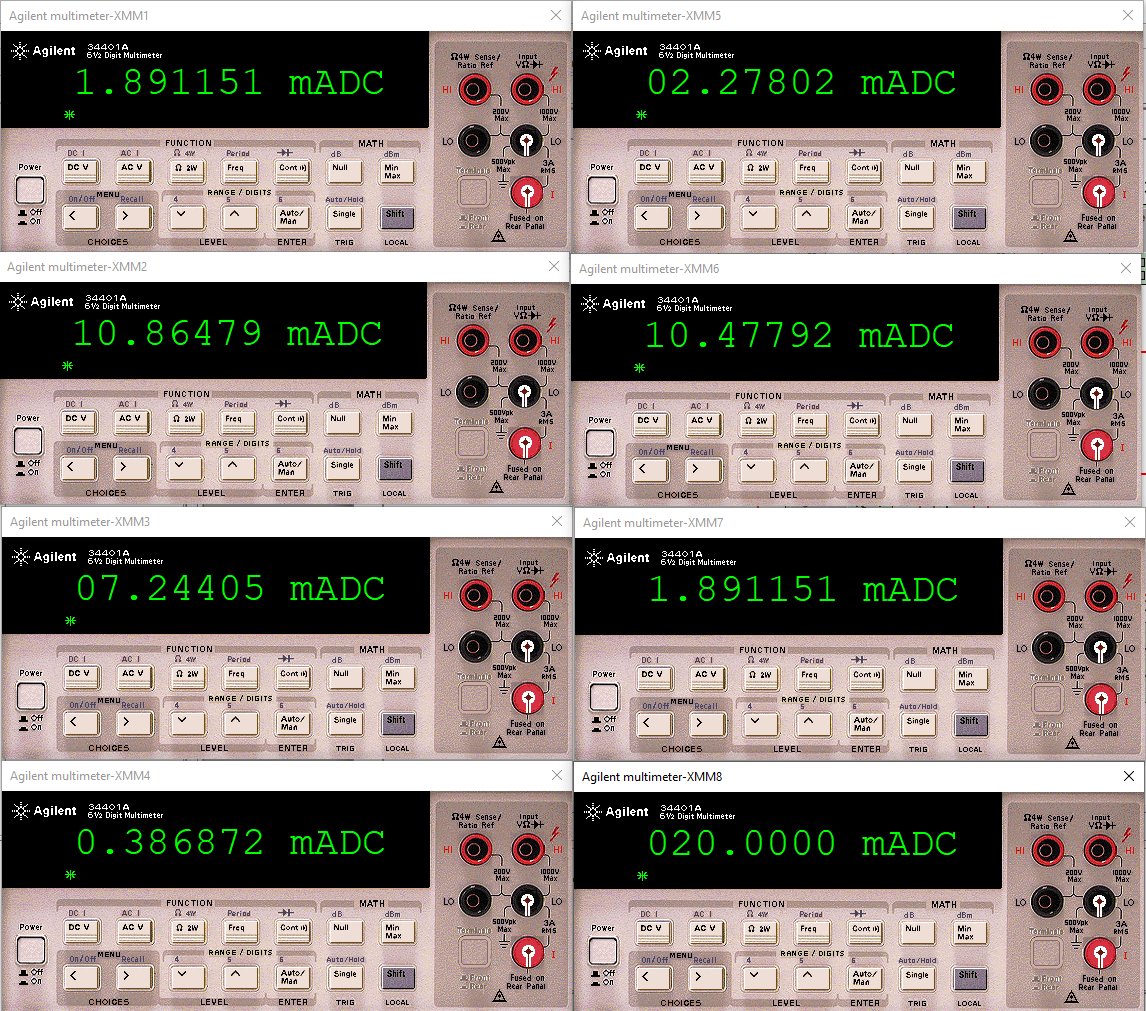
\includegraphics[scale=0.4]{corrientes medidas.PNG}
    \label{fig:my_label}
\end{figure}



\newpage
%%%4%%%



\item Aplicando el teorema de Thévenin, medir $R_{eq}$ y $V_{eq}$ en R6

El voltaje equivalente $V_{eq}$ para R6 se mide de la siguiente forma:

\begin{figure}[h!]
    \centering
    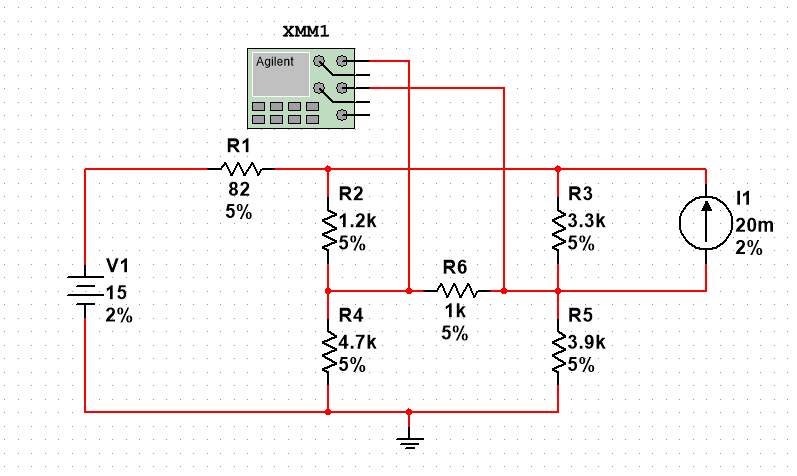
\includegraphics[scale=0.4]{T1.PNG}
    \label{fig:my_label}
\end{figure}


\begin{figure}[h!]
    \centering
    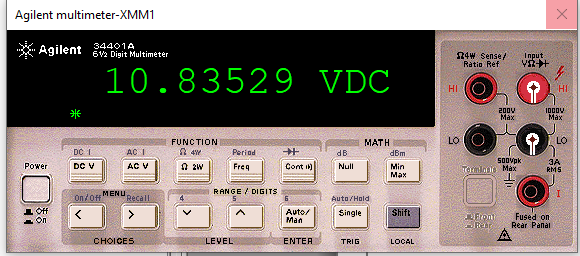
\includegraphics[scale=0.5]{T1.multi.PNG}
    \label{fig:my_label}
\end{figure}

Para medir la resistencia equivalente $R_{eq}$ en R6 se deben quitar todas las fuentes de voltaje y corriente del circuito.

\begin{figure}[h!]
    \centering
    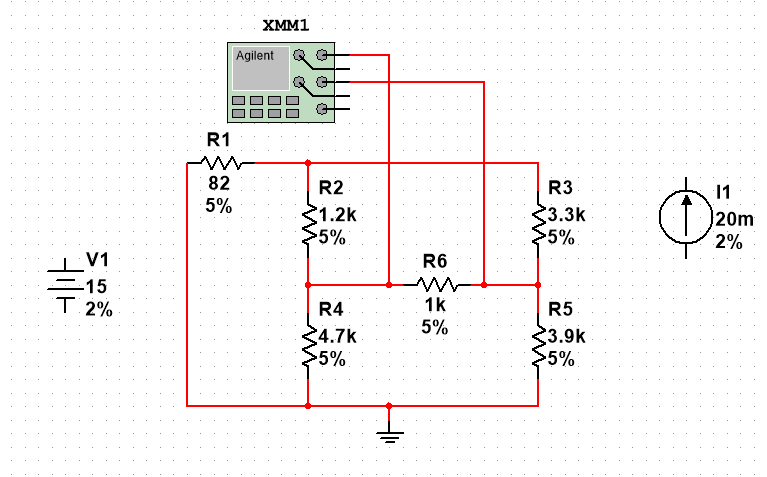
\includegraphics[scale=0.4]{T2.PNG}
    \label{fig:my_label}
\end{figure}

\begin{figure}[h!]
    \centering
    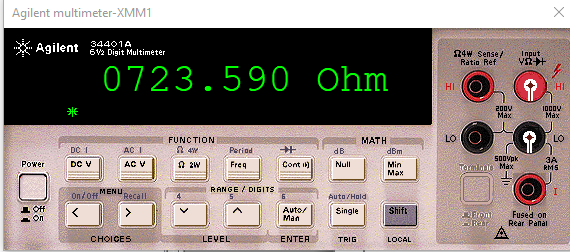
\includegraphics[scale=0.5]{T2.multi.PNG}
    \label{fig:my_label}
\end{figure}


\newpage
%%%5%%%



\item Aplicando el teorema de Norton, medir $R_{eq}$ y $I_{eq}$ en R6

Midiendo la corriente equivalente $I_{eq}$ con el multímetro en paralelo:

\begin{figure}[h!]
    \centering
    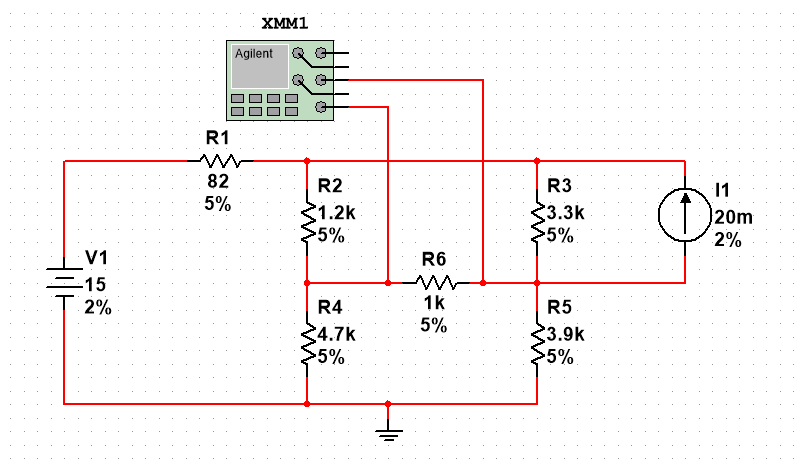
\includegraphics[scale=0.4]{N1.PNG}
    \label{fig:my_label}
\end{figure}

\begin{figure}[h!]
    \centering
    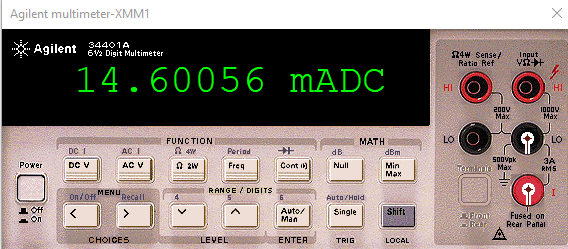
\includegraphics[scale=0.5]{N1.multi.PNG}
    \label{fig:my_label}
\end{figure}

y de nuevo la resistencia equivalente $R_{eq}$:

\begin{figure}[h!]
    \centering
    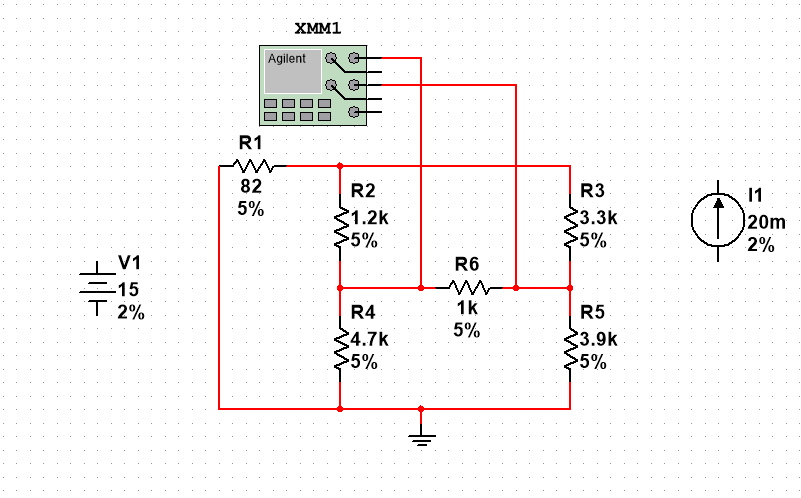
\includegraphics[scale=0.4]{N2.PNG}
    \label{fig:my_label}
\end{figure}

\begin{figure}[h!]
    \centering
    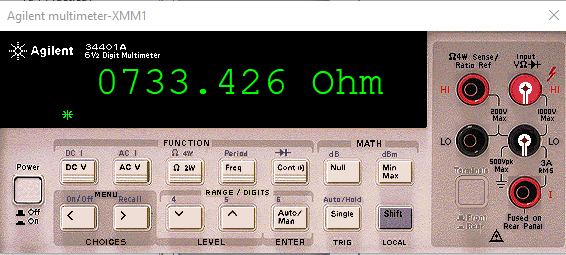
\includegraphics[scale=0.5]{N2.multi.PNG}
    \label{fig:my_label}
\end{figure}

Multiplicando la intensidad equivalente $I_{eq}$ por la resistencia equivalente $R_{eq}$:

\begin{equation*}
    [(14.6005 \pm 0.07) mA] \cdot [(733.426 \pm 0.014) \Omega] = (10.708\pm 0.010) V
\end{equation*}

con un error relativo de $1.2\%$ comparado con lo medido en el objetivo anterior y con el error siendo 13 veces la incertidumbre absoluta.

    
    
\end{enumerate}

\end{document}